\documentclass[12pt,letterpaper]{article}
\usepackage[top=2cm,left=2cm,right=2cm,bottom=2cm]{geometry}
\usepackage[utf8]{inputenc}
\usepackage[T1]{fontenc}  
\usepackage{ae}               % Fonte "Almost European"
\usepackage{amsmath,amssymb}
\usepackage{setspace}
\usepackage{graphicx}
\usepackage{indentfirst}
\usepackage{url}
\usepackage{color}
\usepackage{cite}
\usepackage{gensymb}
\usepackage{subcaption}
\usepackage{hyperref}
\usepackage{epigraph}
\usepackage{mathtools}
\usepackage{mathrsfs}

\definecolor{red}{rgb}{1.0,0.0,0.0}
\definecolor{green}{rgb}{0.01,0.75,0.24}
\definecolor{blue}{rgb}{0.0,0.0,1.0}

\newcommand{\ket}[1]{| #1 \rangle}
\newcommand{\bra}[1]{\langle #1 |}
\newcommand{\expected}[1]{ \langle #1 \rangle}
\newcommand{\product}[2]{\langle #1 | #2 \rangle}
\newcommand{\pib}{\boldsymbol{\pi}}
\newcommand{\sigmab}{\boldsymbol{\sigma}}
\newcommand{\project}{\large Research Project Request  \vskip 0.1cm}
\newcommand{\asu}{Physics Department \\ Arizona State University}

\begin{document}
\onehalfspacing
%\doublespace
\title{\project {\Large \textbf{Quantum Monte Carlo Calculations of Nucleon Systems and Cold Atom Gases}} \vspace{0cm}}
\author{
{\bf PIs: Kevin E. Schmidt}, Arizona State University \\
{\bf Stefano Gandolfi}, Los Alamos National Laboratory
}
\date{\today}
\maketitle

\section*{Abstract}

This research project request is for 500,000 SUs on Stampede. We will use 
Quantum Monte Carlo methods to study nucleon systems and cold atom gases. 
One of our goals is to include explicitly the pionic degrees of freedom in 
the simulations. We also plan to study vortex excitations in both cold atom 
gases and low-density neutron matter. Our large-scale highly-parallel code 
has been successfully used to calculate properties of nuclear matter, 
neutron matter and medium-mass nuclei in the past.

\section{Research Objectives}

This allocation request is intended to provide the computational resources 
to carry out the project \textit{Quantum Monte Carlo (QMC) Calculations of 
Nucleon Systems} supported by the National Science Foundation grant 
PHY-1404405, and related projects.

Many nuclear processes in our universe occur under extreme conditions in 
supernovae and neutron stars. The properties of nuclei and nuclear matter 
under these conditions, which are difficult or impossible to reproduce in 
the laboratory, must necessarily be calculated theoretically. These data are 
needed to understand astrophysically important systems and processes such as 
neutron rich matter, neutron stars, supernovae, and r-process 
nucleosynthesis and neutrino scattering. The quantum many-particle methods 
developed within this project have broad applications across many areas of 
physics, including nuclear physics, cold atomic gas research, and electronic structure. Methods 
previously developed within this project have been applied in each of these 
areas.

The results of this project are relevant for the nuclear physics program at 
the Department of Energy Office of Science, that has identified the 
knowledge of the structure of nuclei and nuclear matter as one of the most 
important scientific questions in nuclear physics in the most recent Nuclear 
Science Advisory Committee long-range plan. This proposal consists mainly of 
two projects, which we describe in the following sections.

%\subsection{QMC simulations with explicit contributions from the pion field}
\subsection{Improved QMC simulations for nuclei and nuclear matter}


Most QMC simulations of nuclear matter model particles interacting via
instantaneous two- and three-body
potentials \cite{car15}. Usually these potentials are derived from chiral 
effective field theories for nuclear structure by approximately integrating 
out the field
degrees of freedom. Our goal is to include explicitly the low energy degrees 
of freedom of the pion field in the QMC
simulations, while the high energy degrees of freedom will be included in 
the instantaneous potentials. We will develop an expression for the low 
energy components of the pion field, the potential for the high energy 
degrees of freedom, the Hamiltonian of the system and suitable wavefunctions 
for this problem.

In QMC the results are highly dependent on the accuracy of the wave function. Currently the trial wave function is only correlated up to linear order as in \cite{gan14}. We will be including quadratic correlations to the trial wave functions of nuclei and nuclear matter.

\subsection{Strongly paired fermionic systems: cold atoms and neutron 
matter}

Strongly paired fermions are important in many contexts, for example cold 
Fermi atom experiments and low-density neutron
matter \cite{gez08,gez10}.
Developing a quantitative understanding of strongly paired
Fermi systems is important since they are a unique
regime for quantum many-body physics.
Cold atom experiments can provide direct tests of the
equation of state and the pairing gap in the strongly
paired regime, and provide a benchmark
of many-body theories in these systems.

Ultracold atomic gases and low-density neutron matter are unique in the 
sense that both exhibit pairing gaps of the order of the Fermi energy 
\cite{bro13}. The neutron scattering length is about -18.5 fm which is 
significantly larger than the interparticle spacing and the interaction 
range 2.7 fm, therefore low density neutron matter is near unitarity. In 
this regime both dilute cold fermion atoms and neutron matter have similar 
properties \cite{car12}. The possibility of tuning particle-particle 
interactions experimentally in cold atomic gases provides an emulation of 
low-density neutron matter, which is beyond direct experimental reach. We 
have studied the vortex structure in cold atomic gases \cite{mad15}
and we intend to extended these calculations to direct simulations of 
vortices in superfluid neutron matter using nuclear Hamiltonians.

Superfluidity of neutron matter is of great interest across astrophysics, 
nuclear physics and many-body physics \cite{gan09}. The occurrence of 
superfluidity in neutron matter is one of many examples of pairing effects 
in low-density many-fermion systems. One signature of superfluidity is the 
formation of quantized vortices and many questions remain to be answered 
concerning the structure of the vortex core in neutron matter. This project 
will be to simulate vortex excitations in superfluid neutron matter using 
QMC methods. Possible properties to be calculated are the vortex excitation 
energy, the superfluid pairing gap and the equation of state.

\section{Computational Methods}
\label{sec:comp_met}

We will use QMC methods, in particular Auxiliary Field Diffusion Monte Carlo 
(AFDMC) methods, which have proven to be very successful in calculating 
ground state properties including momentum distributions, as we have shown 
in our article for Reviews of Modern Physics \cite{car15}. The AFDMC code 
has been successfully used to calculate properties of nuclear matter, 
neutron matter, and medium-mass nuclei \cite{gan14}. The results of 
\cite{gan12} showed the relation between the symmetry energy and properties 
of neutron stars.

We have written a large-scale highly-parallel code to achieve high precision 
calculations for many properties of medium-mass nuclei. The AFDMC code 
calculates the
ground-state of the nucleus through a branching random walk algorithm, and 
can be used to compute other properties including radii and momentum 
distributions.

\subsection{Algorithm and implementation}

The AFDMC code has been developed by the investigators of this project. The 
AFDMC method is used to extract the ground-state component of the system 
from the variational ansatz describing the system. This is done with a 
projection in imaginary-time, i.e. we calculate
\begin{equation}
\label{eq:dif}
\lim_{n\rightarrow\infty}\left[ e^{-H\delta\tau}\right]^n \Psi_T(R,S) 
\rightarrow \Psi_0(R',S'),
\end{equation}
where $R =(r_1, \cdots, r_N)$ are the coordinates of nucleons, $S = (s_1, 
\cdots, s_N)$ are complex numbers indicating their spin and isospin 
projections, and $\Psi_T(R,S)$ is a trial variational wave function. The 
algorithm is a branching random walk that requires the diagonalization of 
$3N \times 3N$ matrices ($N$ is the number of particles) at each step of the 
random walk. AFDMC is written in Fortran90 and MPI, and uses the vendor 
optimized BLAS and LAPACK libraries to perform matrix diagonalizations at 
each step.

The AFDMC algorithm is a variant of Diffusion Monte Carlo, where each step 
involves:
\begin{enumerate}
\item Diffuse nucleon’s positions, $R \rightarrow R'$ according to the 
kinetic energy $T$ of the Hamiltonian.
\item Rotate nucleon’s spins, $S \rightarrow S'$, according to the spin and 
isospin-dependent potential.
\item Calculate the weight $W$ of the new configuration, and generate $N$ 
replicas of the new configuration according to $N = [W + \eta]$, where 
$\eta$  is a random number uniformly distributed from 0 to 1.
\end{enumerate}

This algorithm is implemented by considering
a collection of configurations (called \textit{walkers})
that are simultaneously evolved in imaginary-time. The parallelization is 
accomplished
by spreading the configurations among the nodes. However, AFDMC is not 
embarrassingly parallel because the branching term generates fluctuations in 
the number of configurations, of the order up to 10\%, and the calculation 
of observables requires an average over walkers at the same imaginary-time. 
We employ a dynamic load rebalancing after
each time step to redistribute walkers across nodes.

\section{Application efficiencies}

The AFDMC code is written in Fortran90 and MPI. We describe in detail the 
performance and scaling of our code in the additional document submitted 
with this proposal. The most relevant feature that we present in that 
document is the scaling in Stampede.

We used our startup allocation (TG-PHY140003, PI Kevin Schmidt) to test the 
performance of the code on Stampede. Up to 4096 cores, the 
largest number tested, the code scales strongly. We intend to perform 
simulations with a maximum number of 1024 cores.

\begin{figure}[h]
   \centering
   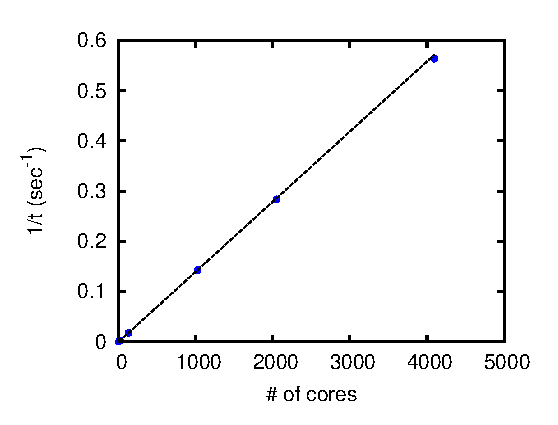
\includegraphics[width=0.7\textwidth]{stampede}
   \caption{Scaling on Stampede using the time to propagate 10000 configurations of an $^{16}O$ nucleus for 100 steps.}
   \label{fig:scaling}
\end{figure}

\section{Computational Research Plan and Justification for Requested 
Resources}

As discussed in Sec. \ref{sec:comp_met}, the simulations depend on a trial 
variational wave function. The variational parameters are determined using 
the stochastic reconfiguration method \cite{cas04}. Once these parameters 
are determined, we can proceed with the computation of physical quantities 
of interest.

%\subsection{QMC simulations with explicit contributions from the pion field}
\subsection{Improved QMC simulations for nuclei and nuclear matter}

We base our estimates on the amount of SUs and storage used in \cite{car15} 
and references therein. We want to perform simulations with different system 
sizes, ranging from one nucleon plus the pion field up to four nucleons plus 
the pion field, a total of four systems. For each system we require:
\begin{itemize}
	\item variational optimization of the parameters: for these systems the 
	average amount of SUs necessary for the optimization is approximately 
	20,000 SUs.
	\item production runs: longer runs are necessary to compute quantities 
	such as energy of the system, density and other distribution functions, 
	with small variances. We estimate 50,000 SUs for these computations.
\end{itemize}

\subsection{Strongly paired fermionic systems}

We base our estimates on the amount of SUs and storage used in \cite{mad15}, 
the most similar calculation in terms of computational cost. We want to 
perform simulations with different system sizes, for example 10 different 
systems with the number of particles varying between 38 and 66 particles. We 
would also like to vary the interaction strength between particles, for 10 
different values of the interaction strength. Hence the total would be of 
100 different systems. For each system we require:
\begin{itemize}
	\item variational optimization of the parameters: for these systems 
	sizes the number of parameters is between 20 and 40 parameters, and the 
	average amount of SUs necessary for the optimization is approximately 
	400 SUs.
	\item production runs: longer runs are necessary to compute quantities 
	such as energy of the system, density and other distribution functions, 
	with small variances. We estimate 1,500 SUs for these computations.
\end{itemize}

\subsection{Summary of the requested resources}

We present in Table \ref{tab:SUs} the amount of SUs requested for each task.
We are requesting a total of 500,000 SUs on Stampede.
The systems of the \textit{Explicit pion field} project require more 
computation time (approximately 50 times the variational optimization and 30 
times for the production runs) than the systems of the \textit{Strongly 
paired fermionic systems} because of extra degrees of freedom. In Eq. 
\ref{eq:dif} we have the $S$ coordinates corresponding to spin and isospin 
projections. These only need to be sampled for the first project, thus the 
difference in computation times. We also included SUs for the code 
development, in order to ensure performance and scaling during execution.

\begin{table}[htbp]
\center
\caption{Justification for the requested amount of SUs}
\begin{tabular}{|l|c|c|}
\hline
 & \multicolumn{1}{l|}{Explicit pion field} & \multicolumn{1}{l|}{Strongly 
 paired fermionic systems} \\ \hline\hline
Development & 20,000 & 10,000 \\ \hline
Variational optimization & 80,000 & 40,000 \\ \hline
Production & 200,000 & 150,000 \\ \hline
Subtotal & 300,000 & 200,000 \\ \hline\hline
\multicolumn{ 3}{|c|}{\textbf{Total: 500,000 SUs}} \\ \hline
\end{tabular}
\label{tab:SUs}
\end{table}

As for storage needs, we request the default value. The size of input, 
output and configuration files is of approximately 50 Mb per system. As the 
simulations are independent, there is no need to store all of them at the 
same time at Stampede. We are capable of handling the post-processing of the 
simulations in our local computing environment.

\section{Additional considerations}

We believe that we have enough funding, through the NSF grant, and qualified 
staff to complete the work plan described in this project.

\subsection{Qualifications of the PIs and team}

\textbf{PIs}

\underline{Kevin Schmidt}

{\color{red} update} \underline{Stefano Gandolfi} is a nationally and 
internationally recognized scientist in Many-Body Nuclear Theory. During the 
past 4 years he has published 25 papers and given 34 invited talks, 
including many at major national and international conferences. He has about 
1,400 citations on Google Scholar. As a result of his excellent work, 
Gandolfi received the International Union of Pure and Applied Physics prize 
for young researchers in nuclear physics in 2013. He has led a program in 
Quantum Monte Carlo at the Institute of Nuclear Theory in 2013.

\textbf{Graduate students}

\underline{Lucas Madeira} is a PhD student at Arizona State University. He 
received his Bachelor degree and Masters degree in Physics from the 
University of Campinas, Brazil. He has experience with High Performance 
Computing including MPI and OpenMP.

\underline{Cody Petrie} is a PhD student at Arizona State University. He received a BS in Physics from Brigham Young University in 2014. He has been computational nuclear physics for the past year and a half.

\newpage
\bibliographystyle{unsrt}
\bibliography{xsede}
\end{document}
